\subsection{Harmonizer}

Harmonizer is structure which detunes input signal slightly to get different "players" play
slightly out of tune as it is in the real orchestra. 

In the harmonizer each window is detuned differently to reduce beating effect. This is
as well real life phenomena as the players of the section will not play all the time same amount
out of tune.  
 
\begin{figure}[ht]
\centering
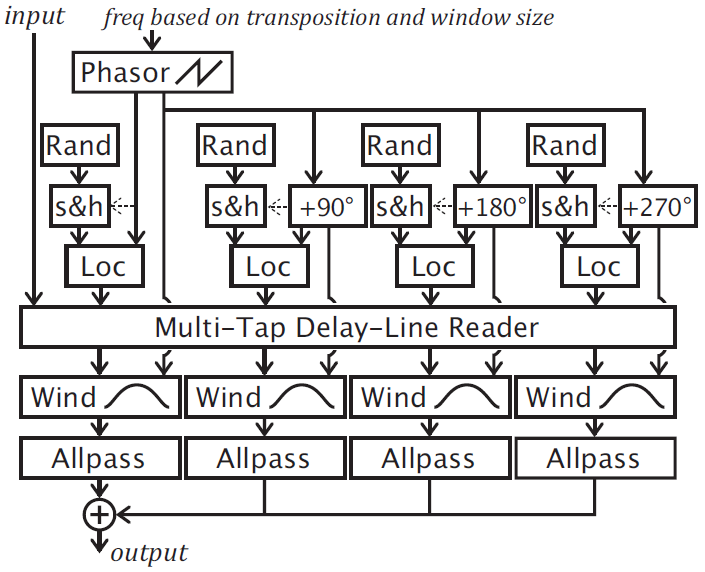
\includegraphics[width = 8cm]{harmonizer.png}
\caption{Chorus Harmonizer Block Diagram. \cite{dudas}}
\label{harm_block}
\end{figure}
